\let\negmedspace\undefined
\let\negthickspace\undefined
\documentclass[journal]{IEEEtran}
\usepackage[a5paper, margin=10mm, onecolumn]{geometry}
%\usepackage{lmodern} % Ensure lmodern is loaded for pdflatex
\usepackage{tfrupee} % Include tfrupee package

\setlength{\headheight}{1cm} % Set the height of the header box
\setlength{\headsep}{0mm}     % Set the distance between the header box and the top of the text

\usepackage{gvv-book}
\usepackage{gvv}
\usepackage{cite}
\usepackage{amsmath,amssymb,amsfonts,amsthm}
\usepackage{algorithmic}
\usepackage{graphicx}
\usepackage{textcomp}
\usepackage{xcolor}
\usepackage{txfonts}
\usepackage{listings}
\usepackage{enumitem}
\usepackage{mathtools}
\usepackage{gensymb}
\usepackage{comment}
\usepackage[breaklinks=true]{hyperref}
\usepackage{tkz-euclide} 
\usepackage{listings}
% \usepackage{gvv}                                        
\def\inputGnumericTable{}                                 
\usepackage[latin1]{inputenc}                                
\usepackage{color}                                            
\usepackage{array}                                            
\usepackage{longtable}                                       
\usepackage{calc}                                             
\usepackage{multirow}                                         
\usepackage{hhline}                                           
\usepackage{ifthen}                                           
\usepackage{lscape}
\begin{document}

\bibliographystyle{IEEEtran}
\vspace{3cm}

\title{CHAPTER - 9\\Differential Equations}
\author{EE24BTECH11061 - Rohith Sai}
% \maketitle
% \newpage
% \bigskip
{\let\newpage\relax\maketitle}

\renewcommand{\thefigure}{\theenumi}
\renewcommand{\thetable}{\theenumi}
\setlength{\intextsep}{10pt} % Space between text and floats

\numberwithin{figure}{enumi}
\renewcommand{\thetable}{\theenumi}

\section*{Exercise : 9.5}
\begin{enumerate}
\item [9)] Solve the differential equation $y dx + x \log{\brak{\frac{y}{x}}} dy - 2x dy = 0$\\
\textbf{Solution:}
The given differential equation is 
\begin{align*}
    y dx + x \log{\brak{\frac{y}{x}}} dy - 2x dy = 0
\end{align*}
On rearranging, we get:
\begin{align}
    \frac{dy}{dx} = \frac{\frac{y}{x}}{2 - \log{\brak{\frac{y}{x}}}}
\end{align}
Let $\frac{y}{x} = v$, i.e., $y = vx$
\begin{align*}
    \implies \frac{dy}{dx} = v + x \frac{dv}{dx}
\end{align*}
Substituting in equation (1), we get:
\begin{align*}
    v + x \frac{dv}{dx} = \frac{v}{2 - \log{v}}\\
    \implies x \frac{dv}{dx} = \frac{v}{2 - \log{v}} - v\\
    \implies x \frac{dv}{dx} = \frac{v \brak{\log{v} - 1}}{2 - \log{v}}\\
    \implies \frac{dx}{x} = \sbrak{\frac{1}{v \brak{\log{v} - 1}} - \frac{1}{v}} dv
\end{align*}
Integrating on both sides, we get:
\begin{align*}
    \log{\abs{x}} + \log{\abs{c}} = \int \sbrak{\frac{1}{v \brak{\log{v} - 1}} - \frac{1}{v}} dv\\
    \implies \log{\abs{x}} + \log{\abs{c}} = \log{\abs{\log{v} - 1}} - \log{\abs{v}}\\
    \implies C x v = \log{v} - 1 \quad \sbrak{\text{where, }C = \pm c} 
\end{align*}
Replacing $v$ by $\frac{y}{x}$ and rearranging, we have:
\begin{align*}
    \log{\brak{\frac{y}{x}}} - 1 = C x \brak{\frac{y}{x}}
\end{align*}
\begin{align}
    \log{\brak{\frac{y}{x}}} - 1 = C y
\end{align}
To obtain a plot for this, let's assume, $C=-1$ and $x = 1$. On substituting these values in equation (2), we get, $y = 1$.\\
Let the $x$ value be limited to 5.
\begin{align*}
    \implies x_0 = 1.0, y_0 = 1.0, x_{end} = 5.0
\end{align*}
The plot of the differential equation 
\begin{align*}
    y dx + x \log{\brak{\frac{y}{x}}} dy - 2x dy = 0
\end{align*}
is shown below.
\begin{figure}[H]
    \centering
    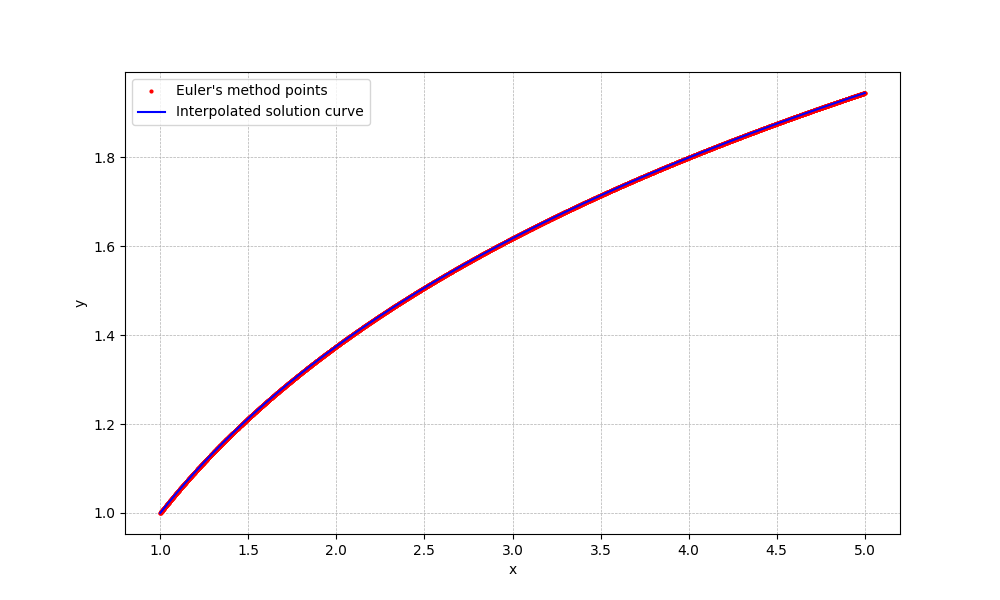
\includegraphics[width = \columnwidth]{figs/fig.png}
\end{figure}
\end{enumerate}
\end{document}